\documentclass[twoside]{book}

% Packages required by doxygen
\usepackage{calc}
\usepackage{doxygen}
\usepackage{graphicx}
\usepackage[utf8]{inputenc}
\usepackage{makeidx}
\usepackage{multicol}
\usepackage{multirow}
\usepackage{textcomp}
\usepackage[table]{xcolor}

% Font selection
\usepackage[T1]{fontenc}
\usepackage{mathptmx}
\usepackage[scaled=.90]{helvet}
\usepackage{courier}
\usepackage{amssymb}
\usepackage{sectsty}
\renewcommand{\familydefault}{\sfdefault}
\allsectionsfont{%
  \fontseries{bc}\selectfont%
  \color{darkgray}%
}
\renewcommand{\DoxyLabelFont}{%
  \fontseries{bc}\selectfont%
  \color{darkgray}%
}

% Page & text layout
\usepackage{geometry}
\geometry{%
  a4paper,%
  top=2.5cm,%
  bottom=2.5cm,%
  left=2.5cm,%
  right=2.5cm%
}
\tolerance=750
\hfuzz=15pt
\hbadness=750
\setlength{\emergencystretch}{15pt}
\setlength{\parindent}{0cm}
\setlength{\parskip}{0.2cm}
\makeatletter
\renewcommand{\paragraph}{%
  \@startsection{paragraph}{4}{0ex}{-1.0ex}{1.0ex}{%
    \normalfont\normalsize\bfseries\SS@parafont%
  }%
}
\renewcommand{\subparagraph}{%
  \@startsection{subparagraph}{5}{0ex}{-1.0ex}{1.0ex}{%
    \normalfont\normalsize\bfseries\SS@subparafont%
  }%
}
\makeatother

% Headers & footers
\usepackage{fancyhdr}
\pagestyle{fancyplain}
\fancyhead[LE]{\fancyplain{}{\bfseries\thepage}}
\fancyhead[CE]{\fancyplain{}{}}
\fancyhead[RE]{\fancyplain{}{\bfseries\leftmark}}
\fancyhead[LO]{\fancyplain{}{\bfseries\rightmark}}
\fancyhead[CO]{\fancyplain{}{}}
\fancyhead[RO]{\fancyplain{}{\bfseries\thepage}}
\fancyfoot[LE]{\fancyplain{}{}}
\fancyfoot[CE]{\fancyplain{}{}}
\fancyfoot[RE]{\fancyplain{}{\bfseries\scriptsize Generated on Tue May 27 2014 19:34:59 for IsFinder by Doxygen }}
\fancyfoot[LO]{\fancyplain{}{\bfseries\scriptsize Generated on Tue May 27 2014 19:34:59 for IsFinder by Doxygen }}
\fancyfoot[CO]{\fancyplain{}{}}
\fancyfoot[RO]{\fancyplain{}{}}
\renewcommand{\footrulewidth}{0.4pt}
\renewcommand{\chaptermark}[1]{%
  \markboth{#1}{}%
}
\renewcommand{\sectionmark}[1]{%
  \markright{\thesection\ #1}%
}

% Indices & bibliography
\usepackage{natbib}
\usepackage[titles]{tocloft}
\setcounter{tocdepth}{3}
\setcounter{secnumdepth}{5}
\makeindex

% Hyperlinks (required, but should be loaded last)
\usepackage{ifpdf}
\ifpdf
  \usepackage[pdftex,pagebackref=true]{hyperref}
\else
  \usepackage[ps2pdf,pagebackref=true]{hyperref}
\fi
\hypersetup{%
  colorlinks=true,%
  linkcolor=blue,%
  citecolor=blue,%
  unicode%
}

% Custom commands
\newcommand{\clearemptydoublepage}{%
  \newpage{\pagestyle{empty}\cleardoublepage}%
}


%===== C O N T E N T S =====

\begin{document}

% Titlepage & ToC
\hypersetup{pageanchor=false}
\pagenumbering{roman}
\begin{titlepage}
\vspace*{7cm}
\begin{center}%
{\Large Is\-Finder \\[1ex]\large 0.\-0.\-1 }\\
\vspace*{1cm}
{\large Generated by Doxygen 1.8.4}\\
\vspace*{0.5cm}
{\small Tue May 27 2014 19:34:59}\\
\end{center}
\end{titlepage}
\clearemptydoublepage
\tableofcontents
\clearemptydoublepage
\pagenumbering{arabic}
\hypersetup{pageanchor=true}

%--- Begin generated contents ---
\chapter{Main Page}
\label{index}\hypertarget{index}{}Is\-Finder finds virus insertion site in host genomic D\-N\-A from pair end N\-G\-S data

\subsection*{Motivation}

\subsection*{Principle}

\subsection*{Get Is\-Finder}

\subsubsection*{From github repository}

``` bash \$ git clone \href{https://github.com/a-slide/IsFinder}{\tt https\-://github.\-com/a-\/slide/\-Is\-Finder} my\-\_\-folder/ ```

\subsubsection*{Archive download}


\begin{DoxyItemize}
\item \href{https://github.com/a-slide/IsFinder/archive/master.zip}{\tt Z\-I\-P archive}
\item \href{https://github.com/a-slide/IsFinder/tarball/master}{\tt T\-A\-R.\-G\-Z archive}
\end{DoxyItemize}

The program must be made executable using {\itshape chmod}. ``` bash \$ sudo chmod u+x Is\-Finder.\-py ```

\subsection*{Usage}

``` bash \$ ./\-Is\-Finder.py ...... ```

\subsubsection*{Dependencies\-:}

The programm was developed under Linux Mint 16 \char`\"{}petra\char`\"{} but is compatible with other L\-I\-N\-U\-X debian based distributions.
\begin{DoxyItemize}
\item python 2.\-7 +
\item Biopython
\end{DoxyItemize}

\subsection*{Pipeline development logbook}


\begin{DoxyItemize}
\item \href{http://nbviewer.ipython.org/github/a-slide/IsFinder/blob/master/doc/Logbook.ipynb}{\tt Logbook}
\end{DoxyItemize}

\subsection*{Authors and Contact}

\href{https://github.com/a-slide}{\tt Adrien Leger} \href{mailto:adrien.leger@gmail.com}{\tt adrien.\-leger@gmail.\-com} 
\chapter{Namespace Index}
\section{Packages}
Here are the packages with brief descriptions (if available)\-:\begin{DoxyCompactList}
\item\contentsline{section}{\hyperlink{namespaceHomologyMasker}{Homology\-Masker} \\*Compared a list of query D\-N\-A sequence with a subject and mask the eventual homologies in the subject sequence with Ns }{\pageref{namespaceHomologyMasker}}{}
\item\contentsline{section}{\hyperlink{namespaceUtilities}{Utilities} \\*Contains several usefull functions to interact with O\-S environement and to parse files }{\pageref{namespaceUtilities}}{}
\end{DoxyCompactList}

\chapter{Hierarchical Index}
\section{Class Hierarchy}
This inheritance list is sorted roughly, but not completely, alphabetically\-:\begin{DoxyCompactList}
\item \contentsline{section}{object}{\pageref{classobject}}{}
\begin{DoxyCompactList}
\item \contentsline{section}{Homology\-Masker.\-Blast}{\pageref{classHomologyMasker_1_1Blast}}{}
\item \contentsline{section}{Homology\-Masker.\-Blast\-Hit}{\pageref{classHomologyMasker_1_1BlastHit}}{}
\item \contentsline{section}{Homology\-Masker.\-Ref\-Masker}{\pageref{classHomologyMasker_1_1RefMasker}}{}
\end{DoxyCompactList}
\end{DoxyCompactList}

\chapter{Class Index}
\section{Class List}
Here are the classes, structs, unions and interfaces with brief descriptions\-:\begin{DoxyCompactList}
\item\contentsline{section}{\hyperlink{classHomologyMasker_1_1Blast}{Homology\-Masker.\-Blast} \\*Singleton class allowing to create a blast database and to perform de blast of a query against a blast database }{\pageref{classHomologyMasker_1_1Blast}}{}
\item\contentsline{section}{\hyperlink{classHomologyMasker_1_1BlastHit}{Homology\-Masker.\-Blast\-Hit} \\*Object oriented class containing information of one blast hit The following instance field are accessible \-: }{\pageref{classHomologyMasker_1_1BlastHit}}{}
\item\contentsline{section}{\hyperlink{classobject}{object} }{\pageref{classobject}}{}
\item\contentsline{section}{\hyperlink{classHomologyMasker_1_1RefMasker}{Homology\-Masker.\-Ref\-Masker} \\*Singleton class allowing to find D\-N\-A sequences homologies between a list of query and a subject and to write a modified version of the subject sequence }{\pageref{classHomologyMasker_1_1RefMasker}}{}
\end{DoxyCompactList}

\chapter{File Index}
\section{File List}
Here is a list of all files with brief descriptions\-:\begin{DoxyCompactList}
\item\contentsline{section}{src/\hyperlink{HomologyMasker_8py}{Homology\-Masker.\-py} }{\pageref{HomologyMasker_8py}}{}
\item\contentsline{section}{src/\hyperlink{Utilities_8py}{Utilities.\-py} }{\pageref{Utilities_8py}}{}
\end{DoxyCompactList}

\chapter{Namespace Documentation}
\hypertarget{namespaceHomologyMasker}{\section{Homology\-Masker Namespace Reference}
\label{namespaceHomologyMasker}\index{Homology\-Masker@{Homology\-Masker}}
}


Compared a list of query D\-N\-A sequence with a subject and mask the eventual homologies in the subject sequence with Ns.  


\subsection*{Classes}
\begin{DoxyCompactItemize}
\item 
class \hyperlink{classHomologyMasker_1_1RefMasker}{Ref\-Masker}
\begin{DoxyCompactList}\small\item\em Singleton class allowing to find D\-N\-A sequences homologies between a list of query and a subject and to write a modified version of the subject sequence. \end{DoxyCompactList}\item 
class \hyperlink{classHomologyMasker_1_1Blast}{Blast}
\begin{DoxyCompactList}\small\item\em Singleton class allowing to create a blast database and to perform de blast of a query against a blast database. \end{DoxyCompactList}\item 
class \hyperlink{classHomologyMasker_1_1BlastHit}{Blast\-Hit}
\begin{DoxyCompactList}\small\item\em Object oriented class containing information of one blast hit The following instance field are accessible \-: \end{DoxyCompactList}\end{DoxyCompactItemize}
\subsection*{Functions}
\begin{DoxyCompactItemize}
\item 
def \hyperlink{namespaceHomologyMasker_a9129003779af13581edac09232ab478c}{masker}
\begin{DoxyCompactList}\small\item\em Main function of \hyperlink{classHomologyMasker_1_1RefMasker}{Ref\-Masker} that integrate database creation, blast and homology masking. \end{DoxyCompactList}\item 
def \hyperlink{namespaceHomologyMasker_a5e2c3f4ec042e879106eb69a8ccff78a}{\-\_\-list\-\_\-homologies}
\begin{DoxyCompactList}\small\item\em Perform iterative blasts of query sequences against the subject database and create a list of hits. \end{DoxyCompactList}\item 
def \hyperlink{namespaceHomologyMasker_a0b05ea350cb75cb8a3e5678491ee8111}{\-\_\-mask\-\_\-homologies}
\begin{DoxyCompactList}\small\item\em Import the reference subject genome, edit it and rewrite an edited version. \end{DoxyCompactList}\item 
def \hyperlink{namespaceHomologyMasker_a7ac860f113bcd1f5179bb296401a0486}{makedb}
\begin{DoxyCompactList}\small\item\em Create a blastn database in subjectdb using makeblastdb. \end{DoxyCompactList}\item 
def \hyperlink{namespaceHomologyMasker_a248ff1fe5259a0e649cbe4fd5f90fe4c}{do\-\_\-blast}
\begin{DoxyCompactList}\small\item\em \hyperlink{classHomologyMasker_1_1Blast}{Blast} query against a subject database and return a list of \hyperlink{classHomologyMasker_1_1BlastHit}{Blast\-Hit} object. \end{DoxyCompactList}\item 
def \hyperlink{namespaceHomologyMasker_af1d8aba7696d25ad2f3053702c6ee6f2}{\-\_\-parse\-\_\-blast}
\item 
def \hyperlink{namespaceHomologyMasker_aa4d7fa9bb74deedda354a794bd261783}{\-\_\-split\-\_\-lines}
\item 
def \hyperlink{namespaceHomologyMasker_ac68e288f6b788691b7124270834c5388}{count\-\_\-total}
\item 
def \hyperlink{namespaceHomologyMasker_ae0d9364665cc50703363a4f90eadb672}{count\-\_\-per\-\_\-ref}
\item 
def \hyperlink{namespaceHomologyMasker_a84b16a475c658df3d9c366a659024166}{get}
\item 
def \hyperlink{namespaceHomologyMasker_a04ee0b72f961634bc42abe3a3be8ed32}{get\-\_\-ref}
\item 
def \hyperlink{namespaceHomologyMasker_a3729ac42a69805ac68804c6a8cf56ac7}{reset\-\_\-list}
\begin{DoxyCompactList}\small\item\em Reset the instance tracking list (Usefull after. \end{DoxyCompactList}\item 
def \hyperlink{namespaceHomologyMasker_abdae33d75b01066dfa3cf9454254479e}{\-\_\-\-\_\-init\-\_\-\-\_\-}
\begin{DoxyCompactList}\small\item\em Create a \hyperlink{classHomologyMasker_1_1BlastHit}{Blast\-Hit} object which is automatically added to the class tracking instance list The object with the following parameters are required for object initialisation. \end{DoxyCompactList}\item 
def \hyperlink{namespaceHomologyMasker_a5de594f4ecece256383cb5c7c0c9fdd2}{\-\_\-\-\_\-repr\-\_\-\-\_\-}
\item 
def \hyperlink{namespaceHomologyMasker_a5a31649f3528f048c1f07c7b26edf091}{\-\_\-\-\_\-str\-\_\-\-\_\-}
\end{DoxyCompactItemize}
\subsection*{Variables}
\begin{DoxyCompactItemize}
\item 
list \hyperlink{namespaceHomologyMasker_af353f622b88a872386648a331c09b7ec}{Instances} = \mbox{[}$\,$\mbox{]}
\item 
\hyperlink{namespaceHomologyMasker_a7ed6087cd5b71af36e04fc7b14404fbf}{q\-\_\-id}
\item 
\hyperlink{namespaceHomologyMasker_ac2f25129910dffef91ae818d733d4dca}{s\-\_\-id}
\item 
\hyperlink{namespaceHomologyMasker_a29c000fdc43af648c175041341b20b7d}{identity}
\item 
\hyperlink{namespaceHomologyMasker_ad039fae339d2981cc166e872097af80a}{length}
\item 
\hyperlink{namespaceHomologyMasker_a1aaaaf3e8d19615bab2d1123a2b815b4}{mis}
\item 
\hyperlink{namespaceHomologyMasker_afba3ae42634f80c7df2f46198386a57a}{gap}
\item 
\hyperlink{namespaceHomologyMasker_a7e1745cc4eda6e4fb742b5bf4da0efd3}{evalue}
\item 
\hyperlink{namespaceHomologyMasker_a615220b802ad22a46f3daea7491caac5}{bscore}
\item 
\hyperlink{namespaceHomologyMasker_a7801a7e7e88a2f65eb24d1bf21ff9e40}{q\-\_\-start}
\item 
\hyperlink{namespaceHomologyMasker_a7ad98af9d6be3028e1cfd7a538636db2}{q\-\_\-end}
\item 
\hyperlink{namespaceHomologyMasker_a65cb71d469b8f9488ed03494375c874d}{s\-\_\-start}
\item 
\hyperlink{namespaceHomologyMasker_a8ee2b993d4ff09d2b322b7511dfad6e9}{s\-\_\-end}
\item 
\hyperlink{namespaceHomologyMasker_ad6a4071a914fba5ea7d3dce772e64064}{q\-\_\-orient}
\item 
\hyperlink{namespaceHomologyMasker_a2d92bc9565ce2b8a00c0d1027f2ef5b7}{s\-\_\-orient}
\end{DoxyCompactItemize}


\subsection{Detailed Description}
Compared a list of query D\-N\-A sequence with a subject and mask the eventual homologies in the subject sequence with Ns. \begin{DoxyCopyright}{Copyright}
\href{http://www.gnu.org/licenses/gpl-2.0.html}{\tt G\-N\-U General Public License v2} 
\end{DoxyCopyright}
\begin{DoxyAuthor}{Author}
Adrien Leger \href{mailto:adrien.leger@gmail.com}{\tt adrien.\-leger@gmail.\-com} 
\end{DoxyAuthor}


\subsection{Function Documentation}
\hypertarget{namespaceHomologyMasker_abdae33d75b01066dfa3cf9454254479e}{\index{Homology\-Masker@{Homology\-Masker}!\-\_\-\-\_\-init\-\_\-\-\_\-@{\-\_\-\-\_\-init\-\_\-\-\_\-}}
\index{\-\_\-\-\_\-init\-\_\-\-\_\-@{\-\_\-\-\_\-init\-\_\-\-\_\-}!HomologyMasker@{Homology\-Masker}}
\subsubsection[{\-\_\-\-\_\-init\-\_\-\-\_\-}]{\setlength{\rightskip}{0pt plus 5cm}def Homology\-Masker.\-\_\-\-\_\-init\-\_\-\-\_\- (
\begin{DoxyParamCaption}
\item[{}]{self, }
\item[{}]{q\-\_\-id, }
\item[{}]{s\-\_\-id, }
\item[{}]{identity, }
\item[{}]{length, }
\item[{}]{mis, }
\item[{}]{gap, }
\item[{}]{q\-\_\-start, }
\item[{}]{q\-\_\-end, }
\item[{}]{s\-\_\-start, }
\item[{}]{s\-\_\-end, }
\item[{}]{evalue, }
\item[{}]{bscore}
\end{DoxyParamCaption}
)}}\label{namespaceHomologyMasker_abdae33d75b01066dfa3cf9454254479e}


Create a \hyperlink{classHomologyMasker_1_1BlastHit}{Blast\-Hit} object which is automatically added to the class tracking instance list The object with the following parameters are required for object initialisation. 


\begin{DoxyParams}{Parameters}
{\em q\-\_\-id} & Query sequence name \\
\hline
{\em s\-\_\-id} & Subject sequence name \\
\hline
{\em identity} & \% of identity in the hit \\
\hline
{\em length} & length of the hit \\
\hline
{\em mis} & Number of mismatch in the hit \\
\hline
{\em gap} & Number of gap in the hit \\
\hline
{\em q\-\_\-start} & Hit start position of the query \\
\hline
{\em q\-\_\-end} & Hit end position of the query \\
\hline
{\em s\-\_\-start} & Hit start position of the subject \\
\hline
{\em s\-\_\-end} & Hit end position of the subject \\
\hline
{\em evalue} & E value of the alignement \\
\hline
{\em bscore} & Bit score of the alignement \\
\hline
\end{DoxyParams}


Definition at line 288 of file Homology\-Masker.\-py.

\hypertarget{namespaceHomologyMasker_a5de594f4ecece256383cb5c7c0c9fdd2}{\index{Homology\-Masker@{Homology\-Masker}!\-\_\-\-\_\-repr\-\_\-\-\_\-@{\-\_\-\-\_\-repr\-\_\-\-\_\-}}
\index{\-\_\-\-\_\-repr\-\_\-\-\_\-@{\-\_\-\-\_\-repr\-\_\-\-\_\-}!HomologyMasker@{Homology\-Masker}}
\subsubsection[{\-\_\-\-\_\-repr\-\_\-\-\_\-}]{\setlength{\rightskip}{0pt plus 5cm}def Homology\-Masker.\-\_\-\-\_\-repr\-\_\-\-\_\- (
\begin{DoxyParamCaption}
\item[{}]{self}
\end{DoxyParamCaption}
)}}\label{namespaceHomologyMasker_a5de594f4ecece256383cb5c7c0c9fdd2}


Definition at line 311 of file Homology\-Masker.\-py.

\hypertarget{namespaceHomologyMasker_a5a31649f3528f048c1f07c7b26edf091}{\index{Homology\-Masker@{Homology\-Masker}!\-\_\-\-\_\-str\-\_\-\-\_\-@{\-\_\-\-\_\-str\-\_\-\-\_\-}}
\index{\-\_\-\-\_\-str\-\_\-\-\_\-@{\-\_\-\-\_\-str\-\_\-\-\_\-}!HomologyMasker@{Homology\-Masker}}
\subsubsection[{\-\_\-\-\_\-str\-\_\-\-\_\-}]{\setlength{\rightskip}{0pt plus 5cm}def Homology\-Masker.\-\_\-\-\_\-str\-\_\-\-\_\- (
\begin{DoxyParamCaption}
\item[{}]{self}
\end{DoxyParamCaption}
)}}\label{namespaceHomologyMasker_a5a31649f3528f048c1f07c7b26edf091}


Definition at line 318 of file Homology\-Masker.\-py.

\hypertarget{namespaceHomologyMasker_a5e2c3f4ec042e879106eb69a8ccff78a}{\index{Homology\-Masker@{Homology\-Masker}!\-\_\-list\-\_\-homologies@{\-\_\-list\-\_\-homologies}}
\index{\-\_\-list\-\_\-homologies@{\-\_\-list\-\_\-homologies}!HomologyMasker@{Homology\-Masker}}
\subsubsection[{\-\_\-list\-\_\-homologies}]{\setlength{\rightskip}{0pt plus 5cm}def Homology\-Masker.\-\_\-list\-\_\-homologies (
\begin{DoxyParamCaption}
\item[{}]{self, }
\item[{}]{query\-\_\-list, }
\item[{}]{subjectdb, }
\item[{}]{evalue}
\end{DoxyParamCaption}
)\hspace{0.3cm}{\ttfamily [private]}}}\label{namespaceHomologyMasker_a5e2c3f4ec042e879106eb69a8ccff78a}


Perform iterative blasts of query sequences against the subject database and create a list of hits. 


\begin{DoxyParams}{Parameters}
{\em query\-\_\-list} & List of paths indicating fasta files containing query sequences. Fasta can contains multiple sequences \\
\hline
{\em subjectdb} & Path of the blastn database of the subject's basename created by \char`\"{}makeblastdb\char`\"{} \\
\hline
{\em evalue} & Cutoff used in blast to select valid hits \\
\hline
\end{DoxyParams}
\begin{DoxyReturn}{Returns}
A list of \hyperlink{classHomologyMasker_1_1BlastHit}{Blast\-Hit} objects 
\end{DoxyReturn}


Definition at line 74 of file Homology\-Masker.\-py.

\hypertarget{namespaceHomologyMasker_a0b05ea350cb75cb8a3e5678491ee8111}{\index{Homology\-Masker@{Homology\-Masker}!\-\_\-mask\-\_\-homologies@{\-\_\-mask\-\_\-homologies}}
\index{\-\_\-mask\-\_\-homologies@{\-\_\-mask\-\_\-homologies}!HomologyMasker@{Homology\-Masker}}
\subsubsection[{\-\_\-mask\-\_\-homologies}]{\setlength{\rightskip}{0pt plus 5cm}def Homology\-Masker.\-\_\-mask\-\_\-homologies (
\begin{DoxyParamCaption}
\item[{}]{self, }
\item[{}]{hit\-\_\-list, }
\item[{}]{subject, }
\item[{}]{output}
\end{DoxyParamCaption}
)\hspace{0.3cm}{\ttfamily [private]}}}\label{namespaceHomologyMasker_a0b05ea350cb75cb8a3e5678491ee8111}


Import the reference subject genome, edit it and rewrite an edited version. 


\begin{DoxyParams}{Parameters}
{\em hit\-\_\-list} & List \hyperlink{classHomologyMasker_1_1BlastHit}{Blast\-Hit} objects descibing the position of hits in the subject sequences \\
\hline
{\em subject} & Path to a fasta file containing the reference subject sequences \\
\hline
{\em output} & Path name of the output subject fasta file \\
\hline
\end{DoxyParams}
\begin{DoxyReturn}{Returns}
A list of \hyperlink{classHomologyMasker_1_1BlastHit}{Blast\-Hit} objects 
\end{DoxyReturn}


Definition at line 93 of file Homology\-Masker.\-py.



Here is the call graph for this function\-:
\nopagebreak
\begin{figure}[H]
\begin{center}
\leavevmode
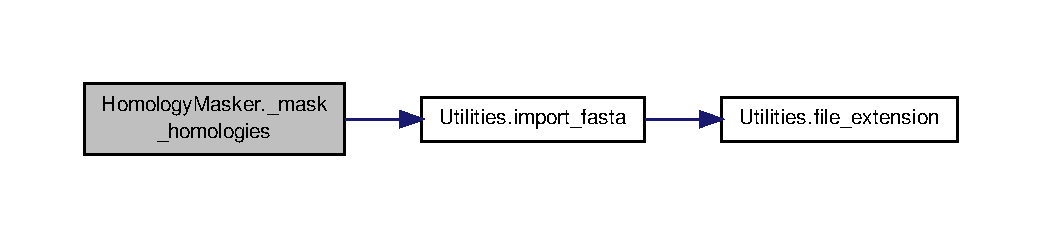
\includegraphics[width=350pt]{namespaceHomologyMasker_a0b05ea350cb75cb8a3e5678491ee8111_cgraph}
\end{center}
\end{figure}


\hypertarget{namespaceHomologyMasker_af1d8aba7696d25ad2f3053702c6ee6f2}{\index{Homology\-Masker@{Homology\-Masker}!\-\_\-parse\-\_\-blast@{\-\_\-parse\-\_\-blast}}
\index{\-\_\-parse\-\_\-blast@{\-\_\-parse\-\_\-blast}!HomologyMasker@{Homology\-Masker}}
\subsubsection[{\-\_\-parse\-\_\-blast}]{\setlength{\rightskip}{0pt plus 5cm}def Homology\-Masker.\-\_\-parse\-\_\-blast (
\begin{DoxyParamCaption}
\item[{}]{self, }
\item[{}]{cmd}
\end{DoxyParamCaption}
)\hspace{0.3cm}{\ttfamily [private]}}}\label{namespaceHomologyMasker_af1d8aba7696d25ad2f3053702c6ee6f2}


Definition at line 183 of file Homology\-Masker.\-py.

\hypertarget{namespaceHomologyMasker_aa4d7fa9bb74deedda354a794bd261783}{\index{Homology\-Masker@{Homology\-Masker}!\-\_\-split\-\_\-lines@{\-\_\-split\-\_\-lines}}
\index{\-\_\-split\-\_\-lines@{\-\_\-split\-\_\-lines}!HomologyMasker@{Homology\-Masker}}
\subsubsection[{\-\_\-split\-\_\-lines}]{\setlength{\rightskip}{0pt plus 5cm}def Homology\-Masker.\-\_\-split\-\_\-lines (
\begin{DoxyParamCaption}
\item[{}]{self, }
\item[{}]{cmd}
\end{DoxyParamCaption}
)\hspace{0.3cm}{\ttfamily [private]}}}\label{namespaceHomologyMasker_aa4d7fa9bb74deedda354a794bd261783}


Definition at line 187 of file Homology\-Masker.\-py.



Here is the call graph for this function\-:
\nopagebreak
\begin{figure}[H]
\begin{center}
\leavevmode
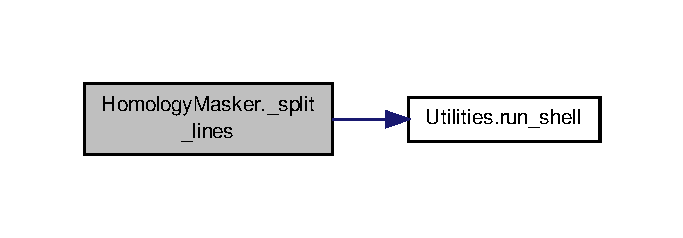
\includegraphics[width=328pt]{namespaceHomologyMasker_aa4d7fa9bb74deedda354a794bd261783_cgraph}
\end{center}
\end{figure}


\hypertarget{namespaceHomologyMasker_ae0d9364665cc50703363a4f90eadb672}{\index{Homology\-Masker@{Homology\-Masker}!count\-\_\-per\-\_\-ref@{count\-\_\-per\-\_\-ref}}
\index{count\-\_\-per\-\_\-ref@{count\-\_\-per\-\_\-ref}!HomologyMasker@{Homology\-Masker}}
\subsubsection[{count\-\_\-per\-\_\-ref}]{\setlength{\rightskip}{0pt plus 5cm}def Homology\-Masker.\-count\-\_\-per\-\_\-ref (
\begin{DoxyParamCaption}
\item[{}]{self}
\end{DoxyParamCaption}
)}}\label{namespaceHomologyMasker_ae0d9364665cc50703363a4f90eadb672}
\begin{DoxyReturn}{Returns}
Number of \hyperlink{classHomologyMasker_1_1BlastHit}{Blast\-Hit} object in Instance list sorted by reference subject sequence 
\end{DoxyReturn}


Definition at line 235 of file Homology\-Masker.\-py.

\hypertarget{namespaceHomologyMasker_ac68e288f6b788691b7124270834c5388}{\index{Homology\-Masker@{Homology\-Masker}!count\-\_\-total@{count\-\_\-total}}
\index{count\-\_\-total@{count\-\_\-total}!HomologyMasker@{Homology\-Masker}}
\subsubsection[{count\-\_\-total}]{\setlength{\rightskip}{0pt plus 5cm}def Homology\-Masker.\-count\-\_\-total (
\begin{DoxyParamCaption}
\item[{}]{self}
\end{DoxyParamCaption}
)}}\label{namespaceHomologyMasker_ac68e288f6b788691b7124270834c5388}
\begin{DoxyReturn}{Returns}
Overall number of \hyperlink{classHomologyMasker_1_1BlastHit}{Blast\-Hit} object in Instance list 
\end{DoxyReturn}


Definition at line 227 of file Homology\-Masker.\-py.

\hypertarget{namespaceHomologyMasker_a248ff1fe5259a0e649cbe4fd5f90fe4c}{\index{Homology\-Masker@{Homology\-Masker}!do\-\_\-blast@{do\-\_\-blast}}
\index{do\-\_\-blast@{do\-\_\-blast}!HomologyMasker@{Homology\-Masker}}
\subsubsection[{do\-\_\-blast}]{\setlength{\rightskip}{0pt plus 5cm}def Homology\-Masker.\-do\-\_\-blast (
\begin{DoxyParamCaption}
\item[{}]{self, }
\item[{}]{query, }
\item[{}]{subjectdb, }
\item[{}]{evalue}
\end{DoxyParamCaption}
)}}\label{namespaceHomologyMasker_a248ff1fe5259a0e649cbe4fd5f90fe4c}


\hyperlink{classHomologyMasker_1_1Blast}{Blast} query against a subject database and return a list of \hyperlink{classHomologyMasker_1_1BlastHit}{Blast\-Hit} object. 


\begin{DoxyParams}{Parameters}
{\em query} & Path to a fasta file containing the query sequences \\
\hline
{\em subjectdb} & Path to the subject blast database basename \\
\hline
{\em evalue} & Cutoff used in blast to select valid hits \\
\hline
\end{DoxyParams}
\begin{DoxyReturn}{Returns}
A list of \hyperlink{classHomologyMasker_1_1BlastHit}{Blast\-Hit} objects if at least one hit was found 
\end{DoxyReturn}

\begin{DoxyExceptions}{Exceptions}
{\em (\-System\-Error,O\-Serror)} & May be returned by run\-\_\-shell in case of invalid command line \\
\hline
\end{DoxyExceptions}


Definition at line 156 of file Homology\-Masker.\-py.



Here is the call graph for this function\-:
\nopagebreak
\begin{figure}[H]
\begin{center}
\leavevmode
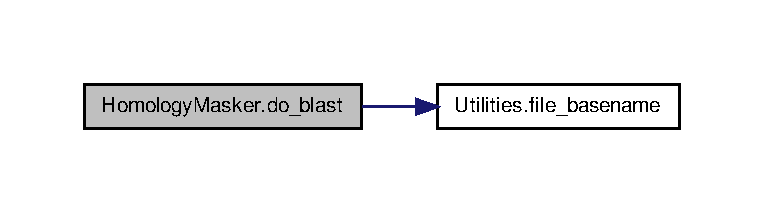
\includegraphics[width=350pt]{namespaceHomologyMasker_a248ff1fe5259a0e649cbe4fd5f90fe4c_cgraph}
\end{center}
\end{figure}


\hypertarget{namespaceHomologyMasker_a84b16a475c658df3d9c366a659024166}{\index{Homology\-Masker@{Homology\-Masker}!get@{get}}
\index{get@{get}!HomologyMasker@{Homology\-Masker}}
\subsubsection[{get}]{\setlength{\rightskip}{0pt plus 5cm}def Homology\-Masker.\-get (
\begin{DoxyParamCaption}
\item[{}]{self}
\end{DoxyParamCaption}
)}}\label{namespaceHomologyMasker_a84b16a475c658df3d9c366a659024166}
\begin{DoxyReturn}{Returns}
The list of all \hyperlink{classHomologyMasker_1_1BlastHit}{Blast\-Hit} object generated 
\end{DoxyReturn}


Definition at line 249 of file Homology\-Masker.\-py.

\hypertarget{namespaceHomologyMasker_a04ee0b72f961634bc42abe3a3be8ed32}{\index{Homology\-Masker@{Homology\-Masker}!get\-\_\-ref@{get\-\_\-ref}}
\index{get\-\_\-ref@{get\-\_\-ref}!HomologyMasker@{Homology\-Masker}}
\subsubsection[{get\-\_\-ref}]{\setlength{\rightskip}{0pt plus 5cm}def Homology\-Masker.\-get\-\_\-ref (
\begin{DoxyParamCaption}
\item[{}]{self, }
\item[{}]{ref}
\end{DoxyParamCaption}
)}}\label{namespaceHomologyMasker_a04ee0b72f961634bc42abe3a3be8ed32}

\begin{DoxyParams}{Parameters}
{\em ref} & Name of a reference sequence in the subject database \\
\hline
\end{DoxyParams}
\begin{DoxyReturn}{Returns}
The list of all \hyperlink{classHomologyMasker_1_1BlastHit}{Blast\-Hit} object generated for this reference 
\end{DoxyReturn}


Definition at line 258 of file Homology\-Masker.\-py.

\hypertarget{namespaceHomologyMasker_a7ac860f113bcd1f5179bb296401a0486}{\index{Homology\-Masker@{Homology\-Masker}!makedb@{makedb}}
\index{makedb@{makedb}!HomologyMasker@{Homology\-Masker}}
\subsubsection[{makedb}]{\setlength{\rightskip}{0pt plus 5cm}def Homology\-Masker.\-makedb (
\begin{DoxyParamCaption}
\item[{}]{self, }
\item[{}]{subject, }
\item[{}]{output}
\end{DoxyParamCaption}
)}}\label{namespaceHomologyMasker_a7ac860f113bcd1f5179bb296401a0486}


Create a blastn database in subjectdb using makeblastdb. 


\begin{DoxyParams}{Parameters}
{\em subject} & Path to a fasta file containing the reference subject sequences \\
\hline
{\em output} & Path to the output database basename \\
\hline
\end{DoxyParams}
\begin{DoxyReturn}{Returns}
Raw output of makeblastdb 
\end{DoxyReturn}

\begin{DoxyExceptions}{Exceptions}
{\em (\-System\-Error,O\-Serror)} & May be returned by run\-\_\-shell in case of invalid command line \\
\hline
\end{DoxyExceptions}


Definition at line 138 of file Homology\-Masker.\-py.



Here is the call graph for this function\-:
\nopagebreak
\begin{figure}[H]
\begin{center}
\leavevmode
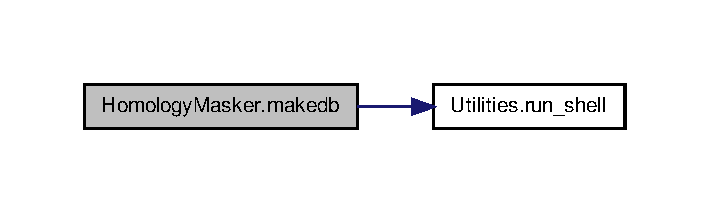
\includegraphics[width=340pt]{namespaceHomologyMasker_a7ac860f113bcd1f5179bb296401a0486_cgraph}
\end{center}
\end{figure}


\hypertarget{namespaceHomologyMasker_a9129003779af13581edac09232ab478c}{\index{Homology\-Masker@{Homology\-Masker}!masker@{masker}}
\index{masker@{masker}!HomologyMasker@{Homology\-Masker}}
\subsubsection[{masker}]{\setlength{\rightskip}{0pt plus 5cm}def Homology\-Masker.\-masker (
\begin{DoxyParamCaption}
\item[{}]{self, }
\item[{}]{query\-\_\-list, }
\item[{}]{subject, }
\item[{}]{evalue, }
\item[{}]{subjectdb = {\ttfamily ''}}
\end{DoxyParamCaption}
)}}\label{namespaceHomologyMasker_a9129003779af13581edac09232ab478c}


Main function of \hyperlink{classHomologyMasker_1_1RefMasker}{Ref\-Masker} that integrate database creation, blast and homology masking. 


\begin{DoxyParams}{Parameters}
{\em query\-\_\-list} & List of paths indicating fasta files containing query sequences. Fasta can contains multiple sequences \\
\hline
{\em subject} & Path to a fasta file containing the reference subject sequences \\
\hline
{\em evalue} & Cutoff used in blast to select valid hits \\
\hline
{\em subjectdb} & Facultative paramater. Path of the blastn database of the subject's basename created by \char`\"{}makeblastdb\char`\"{} \\
\hline
\end{DoxyParams}
\begin{DoxyReturn}{Returns}
If the sequence was edited the path of the edited reference is indicated, else False 
\end{DoxyReturn}


Definition at line 42 of file Homology\-Masker.\-py.



Here is the call graph for this function\-:
\nopagebreak
\begin{figure}[H]
\begin{center}
\leavevmode
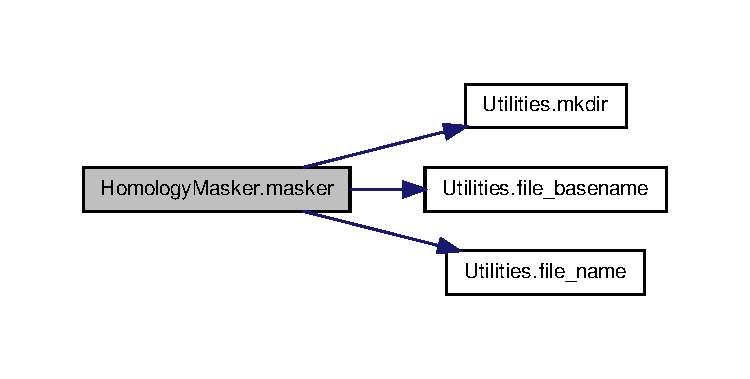
\includegraphics[width=350pt]{namespaceHomologyMasker_a9129003779af13581edac09232ab478c_cgraph}
\end{center}
\end{figure}


\hypertarget{namespaceHomologyMasker_a3729ac42a69805ac68804c6a8cf56ac7}{\index{Homology\-Masker@{Homology\-Masker}!reset\-\_\-list@{reset\-\_\-list}}
\index{reset\-\_\-list@{reset\-\_\-list}!HomologyMasker@{Homology\-Masker}}
\subsubsection[{reset\-\_\-list}]{\setlength{\rightskip}{0pt plus 5cm}def Homology\-Masker.\-reset\-\_\-list (
\begin{DoxyParamCaption}
\item[{}]{self}
\end{DoxyParamCaption}
)}}\label{namespaceHomologyMasker_a3729ac42a69805ac68804c6a8cf56ac7}


Reset the instance tracking list (Usefull after. 



Definition at line 266 of file Homology\-Masker.\-py.



\subsection{Variable Documentation}
\hypertarget{namespaceHomologyMasker_a615220b802ad22a46f3daea7491caac5}{\index{Homology\-Masker@{Homology\-Masker}!bscore@{bscore}}
\index{bscore@{bscore}!HomologyMasker@{Homology\-Masker}}
\subsubsection[{bscore}]{\setlength{\rightskip}{0pt plus 5cm}Homology\-Masker.\-bscore}}\label{namespaceHomologyMasker_a615220b802ad22a46f3daea7491caac5}


Definition at line 296 of file Homology\-Masker.\-py.

\hypertarget{namespaceHomologyMasker_a7e1745cc4eda6e4fb742b5bf4da0efd3}{\index{Homology\-Masker@{Homology\-Masker}!evalue@{evalue}}
\index{evalue@{evalue}!HomologyMasker@{Homology\-Masker}}
\subsubsection[{evalue}]{\setlength{\rightskip}{0pt plus 5cm}Homology\-Masker.\-evalue}}\label{namespaceHomologyMasker_a7e1745cc4eda6e4fb742b5bf4da0efd3}


Definition at line 295 of file Homology\-Masker.\-py.

\hypertarget{namespaceHomologyMasker_afba3ae42634f80c7df2f46198386a57a}{\index{Homology\-Masker@{Homology\-Masker}!gap@{gap}}
\index{gap@{gap}!HomologyMasker@{Homology\-Masker}}
\subsubsection[{gap}]{\setlength{\rightskip}{0pt plus 5cm}Homology\-Masker.\-gap}}\label{namespaceHomologyMasker_afba3ae42634f80c7df2f46198386a57a}


Definition at line 294 of file Homology\-Masker.\-py.

\hypertarget{namespaceHomologyMasker_a29c000fdc43af648c175041341b20b7d}{\index{Homology\-Masker@{Homology\-Masker}!identity@{identity}}
\index{identity@{identity}!HomologyMasker@{Homology\-Masker}}
\subsubsection[{identity}]{\setlength{\rightskip}{0pt plus 5cm}Homology\-Masker.\-identity}}\label{namespaceHomologyMasker_a29c000fdc43af648c175041341b20b7d}


Definition at line 291 of file Homology\-Masker.\-py.

\hypertarget{namespaceHomologyMasker_af353f622b88a872386648a331c09b7ec}{\index{Homology\-Masker@{Homology\-Masker}!Instances@{Instances}}
\index{Instances@{Instances}!HomologyMasker@{Homology\-Masker}}
\subsubsection[{Instances}]{\setlength{\rightskip}{0pt plus 5cm}Homology\-Masker.\-Instances = \mbox{[}$\,$\mbox{]}}}\label{namespaceHomologyMasker_af353f622b88a872386648a331c09b7ec}


Definition at line 218 of file Homology\-Masker.\-py.

\hypertarget{namespaceHomologyMasker_ad039fae339d2981cc166e872097af80a}{\index{Homology\-Masker@{Homology\-Masker}!length@{length}}
\index{length@{length}!HomologyMasker@{Homology\-Masker}}
\subsubsection[{length}]{\setlength{\rightskip}{0pt plus 5cm}Homology\-Masker.\-length}}\label{namespaceHomologyMasker_ad039fae339d2981cc166e872097af80a}


Definition at line 292 of file Homology\-Masker.\-py.

\hypertarget{namespaceHomologyMasker_a1aaaaf3e8d19615bab2d1123a2b815b4}{\index{Homology\-Masker@{Homology\-Masker}!mis@{mis}}
\index{mis@{mis}!HomologyMasker@{Homology\-Masker}}
\subsubsection[{mis}]{\setlength{\rightskip}{0pt plus 5cm}Homology\-Masker.\-mis}}\label{namespaceHomologyMasker_a1aaaaf3e8d19615bab2d1123a2b815b4}


Definition at line 293 of file Homology\-Masker.\-py.

\hypertarget{namespaceHomologyMasker_a7ad98af9d6be3028e1cfd7a538636db2}{\index{Homology\-Masker@{Homology\-Masker}!q\-\_\-end@{q\-\_\-end}}
\index{q\-\_\-end@{q\-\_\-end}!HomologyMasker@{Homology\-Masker}}
\subsubsection[{q\-\_\-end}]{\setlength{\rightskip}{0pt plus 5cm}Homology\-Masker.\-q\-\_\-end}}\label{namespaceHomologyMasker_a7ad98af9d6be3028e1cfd7a538636db2}


Definition at line 300 of file Homology\-Masker.\-py.

\hypertarget{namespaceHomologyMasker_a7ed6087cd5b71af36e04fc7b14404fbf}{\index{Homology\-Masker@{Homology\-Masker}!q\-\_\-id@{q\-\_\-id}}
\index{q\-\_\-id@{q\-\_\-id}!HomologyMasker@{Homology\-Masker}}
\subsubsection[{q\-\_\-id}]{\setlength{\rightskip}{0pt plus 5cm}Homology\-Masker.\-q\-\_\-id}}\label{namespaceHomologyMasker_a7ed6087cd5b71af36e04fc7b14404fbf}


Definition at line 289 of file Homology\-Masker.\-py.

\hypertarget{namespaceHomologyMasker_ad6a4071a914fba5ea7d3dce772e64064}{\index{Homology\-Masker@{Homology\-Masker}!q\-\_\-orient@{q\-\_\-orient}}
\index{q\-\_\-orient@{q\-\_\-orient}!HomologyMasker@{Homology\-Masker}}
\subsubsection[{q\-\_\-orient}]{\setlength{\rightskip}{0pt plus 5cm}Homology\-Masker.\-q\-\_\-orient}}\label{namespaceHomologyMasker_ad6a4071a914fba5ea7d3dce772e64064}


Definition at line 305 of file Homology\-Masker.\-py.

\hypertarget{namespaceHomologyMasker_a7801a7e7e88a2f65eb24d1bf21ff9e40}{\index{Homology\-Masker@{Homology\-Masker}!q\-\_\-start@{q\-\_\-start}}
\index{q\-\_\-start@{q\-\_\-start}!HomologyMasker@{Homology\-Masker}}
\subsubsection[{q\-\_\-start}]{\setlength{\rightskip}{0pt plus 5cm}Homology\-Masker.\-q\-\_\-start}}\label{namespaceHomologyMasker_a7801a7e7e88a2f65eb24d1bf21ff9e40}


Definition at line 299 of file Homology\-Masker.\-py.

\hypertarget{namespaceHomologyMasker_a8ee2b993d4ff09d2b322b7511dfad6e9}{\index{Homology\-Masker@{Homology\-Masker}!s\-\_\-end@{s\-\_\-end}}
\index{s\-\_\-end@{s\-\_\-end}!HomologyMasker@{Homology\-Masker}}
\subsubsection[{s\-\_\-end}]{\setlength{\rightskip}{0pt plus 5cm}Homology\-Masker.\-s\-\_\-end}}\label{namespaceHomologyMasker_a8ee2b993d4ff09d2b322b7511dfad6e9}


Definition at line 302 of file Homology\-Masker.\-py.

\hypertarget{namespaceHomologyMasker_ac2f25129910dffef91ae818d733d4dca}{\index{Homology\-Masker@{Homology\-Masker}!s\-\_\-id@{s\-\_\-id}}
\index{s\-\_\-id@{s\-\_\-id}!HomologyMasker@{Homology\-Masker}}
\subsubsection[{s\-\_\-id}]{\setlength{\rightskip}{0pt plus 5cm}Homology\-Masker.\-s\-\_\-id}}\label{namespaceHomologyMasker_ac2f25129910dffef91ae818d733d4dca}


Definition at line 290 of file Homology\-Masker.\-py.

\hypertarget{namespaceHomologyMasker_a2d92bc9565ce2b8a00c0d1027f2ef5b7}{\index{Homology\-Masker@{Homology\-Masker}!s\-\_\-orient@{s\-\_\-orient}}
\index{s\-\_\-orient@{s\-\_\-orient}!HomologyMasker@{Homology\-Masker}}
\subsubsection[{s\-\_\-orient}]{\setlength{\rightskip}{0pt plus 5cm}Homology\-Masker.\-s\-\_\-orient}}\label{namespaceHomologyMasker_a2d92bc9565ce2b8a00c0d1027f2ef5b7}


Definition at line 306 of file Homology\-Masker.\-py.

\hypertarget{namespaceHomologyMasker_a65cb71d469b8f9488ed03494375c874d}{\index{Homology\-Masker@{Homology\-Masker}!s\-\_\-start@{s\-\_\-start}}
\index{s\-\_\-start@{s\-\_\-start}!HomologyMasker@{Homology\-Masker}}
\subsubsection[{s\-\_\-start}]{\setlength{\rightskip}{0pt plus 5cm}Homology\-Masker.\-s\-\_\-start}}\label{namespaceHomologyMasker_a65cb71d469b8f9488ed03494375c874d}


Definition at line 301 of file Homology\-Masker.\-py.


\hypertarget{namespaceUtilities}{\section{Utilities Namespace Reference}
\label{namespaceUtilities}\index{Utilities@{Utilities}}
}


Contains several usefull functions to interact with O\-S environement and to parse files.  


\subsection*{Functions}
\begin{DoxyCompactItemize}
\item 
def \hyperlink{namespaceUtilities_abe30502337ec442f49d75fd78adc7363}{run\-\_\-shell}
\begin{DoxyCompactList}\small\item\em Run a command line in the default shell and return the standard output. \end{DoxyCompactList}\item 
def \hyperlink{namespaceUtilities_a47e69754d361d402b51251f2a12fb3cd}{mkdir}
\begin{DoxyCompactList}\small\item\em Create a directory at the indicated path\par
 Reproduce the ability of U\-N\-I\-X \char`\"{}mkdir -\/p\char`\"{} command (ie if the path already exits no exception will be raised). \end{DoxyCompactList}\item 
def \hyperlink{namespaceUtilities_a368add4683bf899fca50bae0f8fd6945}{file\-\_\-basename}
\begin{DoxyCompactList}\small\item\em Return the basename of a file without folder location and extension. \end{DoxyCompactList}\item 
def \hyperlink{namespaceUtilities_a0f30d493c3ef8c9882b561e405ea180c}{file\-\_\-extension}
\begin{DoxyCompactList}\small\item\em Return the extension of a file. \end{DoxyCompactList}\item 
def \hyperlink{namespaceUtilities_a1ee03c6d8c2bb70216b5b62051bb125c}{file\-\_\-name}
\begin{DoxyCompactList}\small\item\em Return the complete name of a file with the extension but without folder location. \end{DoxyCompactList}\item 
def \hyperlink{namespaceUtilities_a2220b507ca12a02ecf7b3fe058247ea6}{dir\-\_\-name}
\begin{DoxyCompactList}\small\item\em Return the complete path where is located the file without the file name. \end{DoxyCompactList}\item 
def \hyperlink{namespaceUtilities_a261d2ca73ac395960d97cf8c6b34ba86}{import\-\_\-fasta}
\begin{DoxyCompactList}\small\item\em Import sequences from a fasta files in a list of biopython Seq\-Record. \end{DoxyCompactList}\end{DoxyCompactItemize}


\subsection{Detailed Description}
Contains several usefull functions to interact with O\-S environement and to parse files. \begin{DoxyCopyright}{Copyright}
\href{http://www.gnu.org/licenses/gpl-2.0.html}{\tt G\-N\-U General Public License v2} 
\end{DoxyCopyright}
\begin{DoxyAuthor}{Author}
Adrien Leger \href{mailto:adrien.leger@gmail.com}{\tt adrien.\-leger@gmail.\-com} 
\end{DoxyAuthor}


\subsection{Function Documentation}
\hypertarget{namespaceUtilities_a2220b507ca12a02ecf7b3fe058247ea6}{\index{Utilities@{Utilities}!dir\-\_\-name@{dir\-\_\-name}}
\index{dir\-\_\-name@{dir\-\_\-name}!Utilities@{Utilities}}
\subsubsection[{dir\-\_\-name}]{\setlength{\rightskip}{0pt plus 5cm}def Utilities.\-dir\-\_\-name (
\begin{DoxyParamCaption}
\item[{}]{path}
\end{DoxyParamCaption}
)}}\label{namespaceUtilities_a2220b507ca12a02ecf7b3fe058247ea6}


Return the complete path where is located the file without the file name. 


\begin{DoxyParams}{Parameters}
{\em path} & Filepath as a string \\
\hline
\end{DoxyParams}


Definition at line 96 of file Utilities.\-py.

\hypertarget{namespaceUtilities_a368add4683bf899fca50bae0f8fd6945}{\index{Utilities@{Utilities}!file\-\_\-basename@{file\-\_\-basename}}
\index{file\-\_\-basename@{file\-\_\-basename}!Utilities@{Utilities}}
\subsubsection[{file\-\_\-basename}]{\setlength{\rightskip}{0pt plus 5cm}def Utilities.\-file\-\_\-basename (
\begin{DoxyParamCaption}
\item[{}]{path}
\end{DoxyParamCaption}
)}}\label{namespaceUtilities_a368add4683bf899fca50bae0f8fd6945}


Return the basename of a file without folder location and extension. 


\begin{DoxyParams}{Parameters}
{\em path} & Filepath as a string \\
\hline
\end{DoxyParams}


Definition at line 72 of file Utilities.\-py.



Here is the caller graph for this function\-:
\nopagebreak
\begin{figure}[H]
\begin{center}
\leavevmode
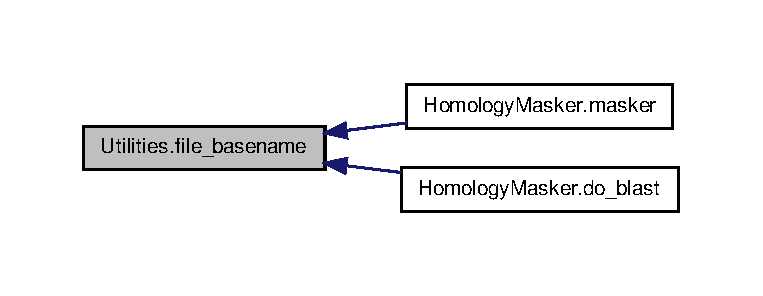
\includegraphics[width=350pt]{namespaceUtilities_a368add4683bf899fca50bae0f8fd6945_icgraph}
\end{center}
\end{figure}


\hypertarget{namespaceUtilities_a0f30d493c3ef8c9882b561e405ea180c}{\index{Utilities@{Utilities}!file\-\_\-extension@{file\-\_\-extension}}
\index{file\-\_\-extension@{file\-\_\-extension}!Utilities@{Utilities}}
\subsubsection[{file\-\_\-extension}]{\setlength{\rightskip}{0pt plus 5cm}def Utilities.\-file\-\_\-extension (
\begin{DoxyParamCaption}
\item[{}]{path}
\end{DoxyParamCaption}
)}}\label{namespaceUtilities_a0f30d493c3ef8c9882b561e405ea180c}


Return the extension of a file. 


\begin{DoxyParams}{Parameters}
{\em path} & Filepath as a string \\
\hline
\end{DoxyParams}


Definition at line 80 of file Utilities.\-py.



Here is the caller graph for this function\-:
\nopagebreak
\begin{figure}[H]
\begin{center}
\leavevmode
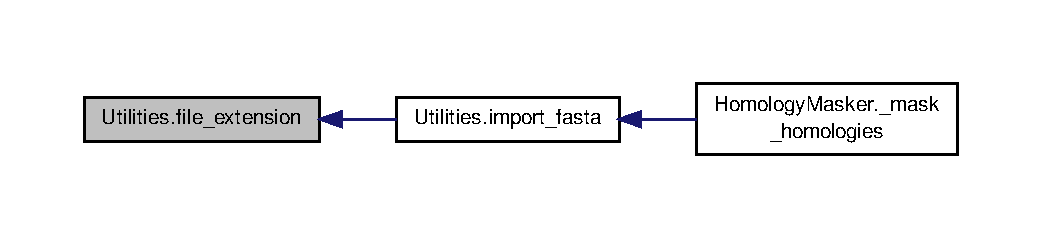
\includegraphics[width=350pt]{namespaceUtilities_a0f30d493c3ef8c9882b561e405ea180c_icgraph}
\end{center}
\end{figure}


\hypertarget{namespaceUtilities_a1ee03c6d8c2bb70216b5b62051bb125c}{\index{Utilities@{Utilities}!file\-\_\-name@{file\-\_\-name}}
\index{file\-\_\-name@{file\-\_\-name}!Utilities@{Utilities}}
\subsubsection[{file\-\_\-name}]{\setlength{\rightskip}{0pt plus 5cm}def Utilities.\-file\-\_\-name (
\begin{DoxyParamCaption}
\item[{}]{path}
\end{DoxyParamCaption}
)}}\label{namespaceUtilities_a1ee03c6d8c2bb70216b5b62051bb125c}


Return the complete name of a file with the extension but without folder location. 


\begin{DoxyParams}{Parameters}
{\em path} & Filepath as a string \\
\hline
\end{DoxyParams}


Definition at line 88 of file Utilities.\-py.



Here is the caller graph for this function\-:
\nopagebreak
\begin{figure}[H]
\begin{center}
\leavevmode
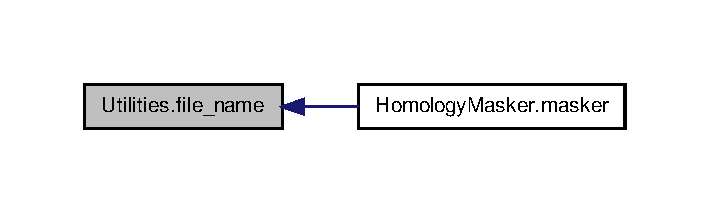
\includegraphics[width=340pt]{namespaceUtilities_a1ee03c6d8c2bb70216b5b62051bb125c_icgraph}
\end{center}
\end{figure}


\hypertarget{namespaceUtilities_a261d2ca73ac395960d97cf8c6b34ba86}{\index{Utilities@{Utilities}!import\-\_\-fasta@{import\-\_\-fasta}}
\index{import\-\_\-fasta@{import\-\_\-fasta}!Utilities@{Utilities}}
\subsubsection[{import\-\_\-fasta}]{\setlength{\rightskip}{0pt plus 5cm}def Utilities.\-import\-\_\-fasta (
\begin{DoxyParamCaption}
\item[{}]{filename, }
\item[{}]{col\-\_\-type = {\ttfamily \char`\"{}dict\char`\"{}}}
\end{DoxyParamCaption}
)}}\label{namespaceUtilities_a261d2ca73ac395960d97cf8c6b34ba86}


Import sequences from a fasta files in a list of biopython Seq\-Record. 


\begin{DoxyParams}{Parameters}
{\em filename} & Valid path to a fasta file (may contains several sequences) \\
\hline
{\em col\-\_\-type} & Type of the collection where Seq\-Reccord entries will be added \char`\"{}list\char`\"{} or \char`\"{}dict\char`\"{}. \\
\hline
\end{DoxyParams}
\begin{DoxyReturn}{Returns}
A list or a dictionnary containing all seq\-Reccord objects from the fastq file 
\end{DoxyReturn}

\begin{DoxyExceptions}{Exceptions}
{\em I\-O\-Error} & Raise if the path in invalid or unreadeable \\
\hline
\end{DoxyExceptions}


Definition at line 109 of file Utilities.\-py.



Here is the call graph for this function\-:
\nopagebreak
\begin{figure}[H]
\begin{center}
\leavevmode
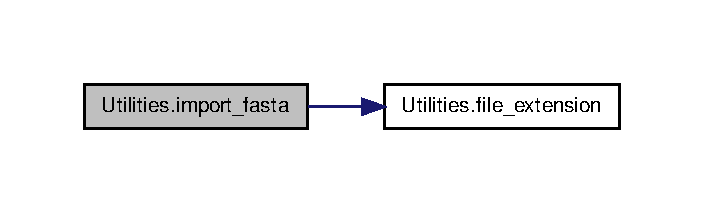
\includegraphics[width=338pt]{namespaceUtilities_a261d2ca73ac395960d97cf8c6b34ba86_cgraph}
\end{center}
\end{figure}




Here is the caller graph for this function\-:
\nopagebreak
\begin{figure}[H]
\begin{center}
\leavevmode
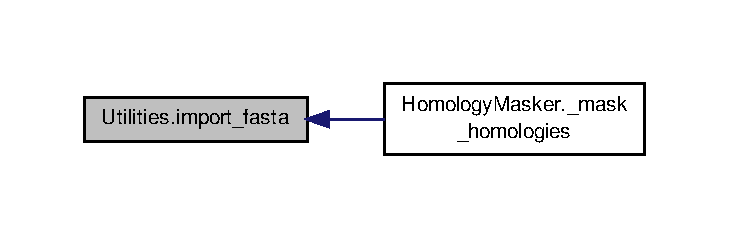
\includegraphics[width=350pt]{namespaceUtilities_a261d2ca73ac395960d97cf8c6b34ba86_icgraph}
\end{center}
\end{figure}


\hypertarget{namespaceUtilities_a47e69754d361d402b51251f2a12fb3cd}{\index{Utilities@{Utilities}!mkdir@{mkdir}}
\index{mkdir@{mkdir}!Utilities@{Utilities}}
\subsubsection[{mkdir}]{\setlength{\rightskip}{0pt plus 5cm}def Utilities.\-mkdir (
\begin{DoxyParamCaption}
\item[{}]{fp}
\end{DoxyParamCaption}
)}}\label{namespaceUtilities_a47e69754d361d402b51251f2a12fb3cd}


Create a directory at the indicated path\par
 Reproduce the ability of U\-N\-I\-X \char`\"{}mkdir -\/p\char`\"{} command (ie if the path already exits no exception will be raised). 


\begin{DoxyParams}{Parameters}
{\em fp} & path name where the folder should be created \\
\hline
\end{DoxyParams}

\begin{DoxyExceptions}{Exceptions}
{\em O\-S\-Error} & Can be raise by os.\-mkdir \\
\hline
\end{DoxyExceptions}


Definition at line 51 of file Utilities.\-py.



Here is the caller graph for this function\-:
\nopagebreak
\begin{figure}[H]
\begin{center}
\leavevmode
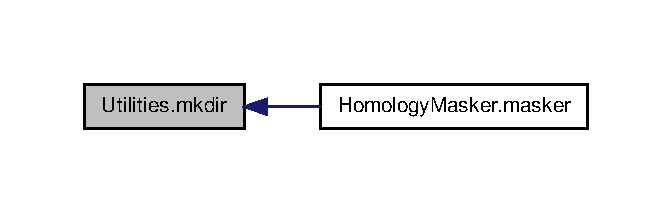
\includegraphics[width=322pt]{namespaceUtilities_a47e69754d361d402b51251f2a12fb3cd_icgraph}
\end{center}
\end{figure}


\hypertarget{namespaceUtilities_abe30502337ec442f49d75fd78adc7363}{\index{Utilities@{Utilities}!run\-\_\-shell@{run\-\_\-shell}}
\index{run\-\_\-shell@{run\-\_\-shell}!Utilities@{Utilities}}
\subsubsection[{run\-\_\-shell}]{\setlength{\rightskip}{0pt plus 5cm}def Utilities.\-run\-\_\-shell (
\begin{DoxyParamCaption}
\item[{}]{cmd}
\end{DoxyParamCaption}
)}}\label{namespaceUtilities_abe30502337ec442f49d75fd78adc7363}


Run a command line in the default shell and return the standard output. 


\begin{DoxyParams}{Parameters}
{\em cmd} & a command line string formated as a string \\
\hline
\end{DoxyParams}
\begin{DoxyReturn}{Returns}
If no standard error return the standard output as a string 
\end{DoxyReturn}

\begin{DoxyExceptions}{Exceptions}
{\em O\-S\-Error} & Raise if a message is return on the standard error output \\
\hline
{\em (\-Value\-Error,O\-S\-Error)} & May be raise by Popen \\
\hline
\end{DoxyExceptions}


Definition at line 19 of file Utilities.\-py.



Here is the caller graph for this function\-:
\nopagebreak
\begin{figure}[H]
\begin{center}
\leavevmode
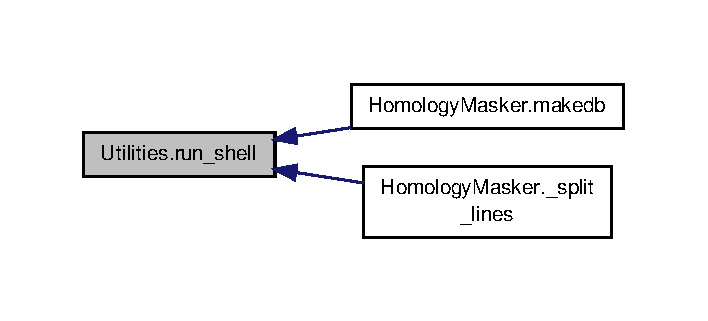
\includegraphics[width=340pt]{namespaceUtilities_abe30502337ec442f49d75fd78adc7363_icgraph}
\end{center}
\end{figure}



\chapter{Class Documentation}
\hypertarget{classHomologyMasker_1_1Blast}{\section{Homology\-Masker.\-Blast Class Reference}
\label{classHomologyMasker_1_1Blast}\index{Homology\-Masker.\-Blast@{Homology\-Masker.\-Blast}}
}


Singleton class allowing to create a blast database and to perform de blast of a query against a blast database.  




Inheritance diagram for Homology\-Masker.\-Blast\-:
\nopagebreak
\begin{figure}[H]
\begin{center}
\leavevmode
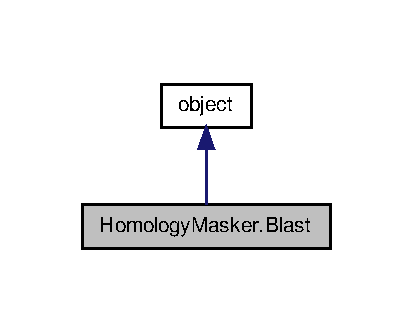
\includegraphics[width=198pt]{classHomologyMasker_1_1Blast__inherit__graph}
\end{center}
\end{figure}


Collaboration diagram for Homology\-Masker.\-Blast\-:
\nopagebreak
\begin{figure}[H]
\begin{center}
\leavevmode
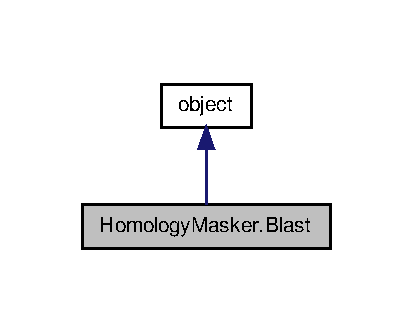
\includegraphics[width=198pt]{classHomologyMasker_1_1Blast__coll__graph}
\end{center}
\end{figure}


\subsection{Detailed Description}
Singleton class allowing to create a blast database and to perform de blast of a query against a blast database. 

Blast+ 2.\-8+ needs to be install and correctly added to the path 

Definition at line 124 of file Homology\-Masker.\-py.



The documentation for this class was generated from the following file\-:\begin{DoxyCompactItemize}
\item 
src/\hyperlink{HomologyMasker_8py}{Homology\-Masker.\-py}\end{DoxyCompactItemize}

\hypertarget{classHomologyMasker_1_1BlastHit}{\section{Homology\-Masker.\-Blast\-Hit Class Reference}
\label{classHomologyMasker_1_1BlastHit}\index{Homology\-Masker.\-Blast\-Hit@{Homology\-Masker.\-Blast\-Hit}}
}


Object oriented class containing information of one blast hit The following instance field are accessible \-:  




Inheritance diagram for Homology\-Masker.\-Blast\-Hit\-:
\nopagebreak
\begin{figure}[H]
\begin{center}
\leavevmode
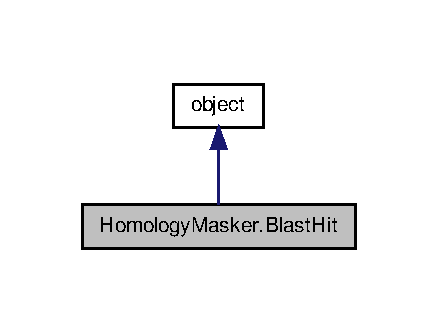
\includegraphics[width=210pt]{classHomologyMasker_1_1BlastHit__inherit__graph}
\end{center}
\end{figure}


Collaboration diagram for Homology\-Masker.\-Blast\-Hit\-:
\nopagebreak
\begin{figure}[H]
\begin{center}
\leavevmode
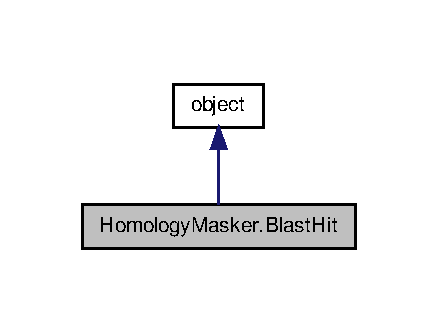
\includegraphics[width=210pt]{classHomologyMasker_1_1BlastHit__coll__graph}
\end{center}
\end{figure}


\subsection{Detailed Description}
Object oriented class containing information of one blast hit The following instance field are accessible \-: 


\begin{DoxyItemize}
\item q\-\_\-id \-: Query sequence name
\item s\-\_\-id \-: Subject sequence name
\item identity \-: \% of identity in the hit
\item length \-: length of the hit
\item mis \-: Number of mismatch in the hit
\item gap \-: Number of gap in the hit
\item q\-\_\-orient \-: Orientation of the query along the hit
\item q\-\_\-start \-: Hit start position of the query
\item q\-\_\-end \-: Hit end position of the query
\item s\-\_\-orient \-: Orientation of the subject along the hit
\item s\-\_\-start \-: Hit start position of the subject
\item s\-\_\-end \-: Hit end position of the subject
\item evalue \-: E value of the alignement
\item b\-\_\-score \-: Bit score of the alignement A class list is used to track all instances generated. 
\end{DoxyItemize}

Definition at line 213 of file Homology\-Masker.\-py.



The documentation for this class was generated from the following file\-:\begin{DoxyCompactItemize}
\item 
src/\hyperlink{HomologyMasker_8py}{Homology\-Masker.\-py}\end{DoxyCompactItemize}

\hypertarget{classobject}{\section{object Class Reference}
\label{classobject}\index{object@{object}}
}


Inheritance diagram for object\-:
\nopagebreak
\begin{figure}[H]
\begin{center}
\leavevmode
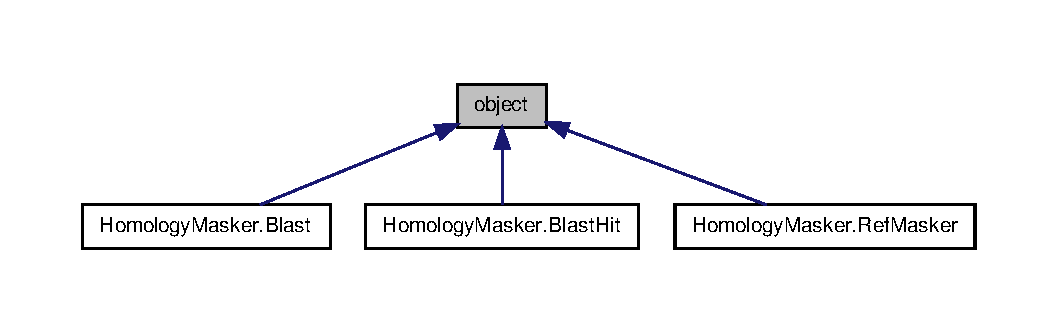
\includegraphics[width=350pt]{classobject__inherit__graph}
\end{center}
\end{figure}


The documentation for this class was generated from the following file\-:\begin{DoxyCompactItemize}
\item 
src/\hyperlink{HomologyMasker_8py}{Homology\-Masker.\-py}\end{DoxyCompactItemize}

\hypertarget{classHomologyMasker_1_1RefMasker}{\section{Homology\-Masker.\-Ref\-Masker Class Reference}
\label{classHomologyMasker_1_1RefMasker}\index{Homology\-Masker.\-Ref\-Masker@{Homology\-Masker.\-Ref\-Masker}}
}


Singleton class allowing to find D\-N\-A sequences homologies between a list of query and a subject and to write a modified version of the subject sequence.  




Inheritance diagram for Homology\-Masker.\-Ref\-Masker\-:
\nopagebreak
\begin{figure}[H]
\begin{center}
\leavevmode
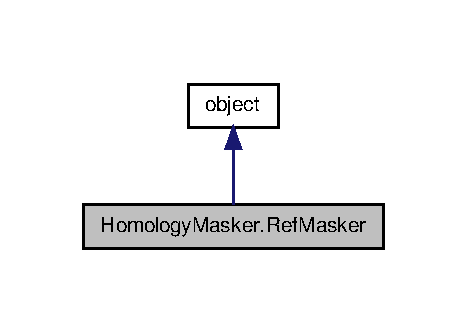
\includegraphics[width=224pt]{classHomologyMasker_1_1RefMasker__inherit__graph}
\end{center}
\end{figure}


Collaboration diagram for Homology\-Masker.\-Ref\-Masker\-:
\nopagebreak
\begin{figure}[H]
\begin{center}
\leavevmode
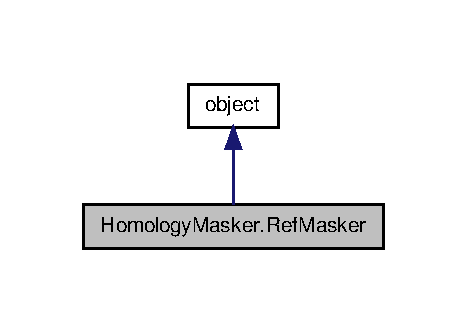
\includegraphics[width=224pt]{classHomologyMasker_1_1RefMasker__coll__graph}
\end{center}
\end{figure}


\subsection{Detailed Description}
Singleton class allowing to find D\-N\-A sequences homologies between a list of query and a subject and to write a modified version of the subject sequence. 

First a blast database is created from a reference fasta file if it is not provided by the user. Then, query sequences fasta files are blasted against the newly created subject database. Finally, if blast hits are found (homologies) the subject genome is imported, hit locations are masked with \char`\"{}\-Ns\char`\"{} and a new masked reference is written 

Definition at line 27 of file Homology\-Masker.\-py.



The documentation for this class was generated from the following file\-:\begin{DoxyCompactItemize}
\item 
src/\hyperlink{HomologyMasker_8py}{Homology\-Masker.\-py}\end{DoxyCompactItemize}

\chapter{File Documentation}
\hypertarget{readme_8md}{\section{readme.\-md File Reference}
\label{readme_8md}\index{readme.\-md@{readme.\-md}}
}

\hypertarget{HomologyMasker_8py}{\section{src/\-Homology\-Masker.py File Reference}
\label{HomologyMasker_8py}\index{src/\-Homology\-Masker.\-py@{src/\-Homology\-Masker.\-py}}
}
\subsection*{Classes}
\begin{DoxyCompactItemize}
\item 
class \hyperlink{classHomologyMasker_1_1RefMasker}{Homology\-Masker.\-Ref\-Masker}
\begin{DoxyCompactList}\small\item\em Singleton class allowing to find D\-N\-A sequences homologies between a list of query and a subject and to write a modified version of the subject sequence. \end{DoxyCompactList}\item 
class \hyperlink{classHomologyMasker_1_1Blast}{Homology\-Masker.\-Blast}
\begin{DoxyCompactList}\small\item\em Singleton class allowing to create a blast database and to perform de blast of a query against a blast database. \end{DoxyCompactList}\item 
class \hyperlink{classHomologyMasker_1_1BlastHit}{Homology\-Masker.\-Blast\-Hit}
\begin{DoxyCompactList}\small\item\em Object oriented class containing information of one blast hit The following instance field are accessible \-: \end{DoxyCompactList}\end{DoxyCompactItemize}
\subsection*{Namespaces}
\begin{DoxyCompactItemize}
\item 
\hyperlink{namespaceHomologyMasker}{Homology\-Masker}
\begin{DoxyCompactList}\small\item\em Compared a list of query D\-N\-A sequence with a subject and mask the eventual homologies in the subject sequence with Ns. \end{DoxyCompactList}\end{DoxyCompactItemize}
\subsection*{Constant Groups}
\begin{DoxyCompactItemize}
\item 
\hyperlink{namespaceHomologyMasker}{Homology\-Masker}
\begin{DoxyCompactList}\small\item\em Compared a list of query D\-N\-A sequence with a subject and mask the eventual homologies in the subject sequence with Ns. \end{DoxyCompactList}\end{DoxyCompactItemize}
\subsection*{Functions}
\begin{DoxyCompactItemize}
\item 
def \hyperlink{namespaceHomologyMasker_a9129003779af13581edac09232ab478c}{Homology\-Masker.\-masker}
\begin{DoxyCompactList}\small\item\em Main function of \hyperlink{classHomologyMasker_1_1RefMasker}{Ref\-Masker} that integrate database creation, blast and homology masking. \end{DoxyCompactList}\item 
def \hyperlink{namespaceHomologyMasker_a5e2c3f4ec042e879106eb69a8ccff78a}{Homology\-Masker.\-\_\-list\-\_\-homologies}
\begin{DoxyCompactList}\small\item\em Perform iterative blasts of query sequences against the subject database and create a list of hits. \end{DoxyCompactList}\item 
def \hyperlink{namespaceHomologyMasker_a0b05ea350cb75cb8a3e5678491ee8111}{Homology\-Masker.\-\_\-mask\-\_\-homologies}
\begin{DoxyCompactList}\small\item\em Import the reference subject genome, edit it and rewrite an edited version. \end{DoxyCompactList}\item 
def \hyperlink{namespaceHomologyMasker_a7ac860f113bcd1f5179bb296401a0486}{Homology\-Masker.\-makedb}
\begin{DoxyCompactList}\small\item\em Create a blastn database in subjectdb using makeblastdb. \end{DoxyCompactList}\item 
def \hyperlink{namespaceHomologyMasker_a248ff1fe5259a0e649cbe4fd5f90fe4c}{Homology\-Masker.\-do\-\_\-blast}
\begin{DoxyCompactList}\small\item\em \hyperlink{classHomologyMasker_1_1Blast}{Blast} query against a subject database and return a list of \hyperlink{classHomologyMasker_1_1BlastHit}{Blast\-Hit} object. \end{DoxyCompactList}\item 
def \hyperlink{namespaceHomologyMasker_af1d8aba7696d25ad2f3053702c6ee6f2}{Homology\-Masker.\-\_\-parse\-\_\-blast}
\item 
def \hyperlink{namespaceHomologyMasker_aa4d7fa9bb74deedda354a794bd261783}{Homology\-Masker.\-\_\-split\-\_\-lines}
\item 
def \hyperlink{namespaceHomologyMasker_ac68e288f6b788691b7124270834c5388}{Homology\-Masker.\-count\-\_\-total}
\item 
def \hyperlink{namespaceHomologyMasker_ae0d9364665cc50703363a4f90eadb672}{Homology\-Masker.\-count\-\_\-per\-\_\-ref}
\item 
def \hyperlink{namespaceHomologyMasker_a84b16a475c658df3d9c366a659024166}{Homology\-Masker.\-get}
\item 
def \hyperlink{namespaceHomologyMasker_a04ee0b72f961634bc42abe3a3be8ed32}{Homology\-Masker.\-get\-\_\-ref}
\item 
def \hyperlink{namespaceHomologyMasker_a3729ac42a69805ac68804c6a8cf56ac7}{Homology\-Masker.\-reset\-\_\-list}
\begin{DoxyCompactList}\small\item\em Reset the instance tracking list (Usefull after. \end{DoxyCompactList}\item 
def \hyperlink{namespaceHomologyMasker_abdae33d75b01066dfa3cf9454254479e}{Homology\-Masker.\-\_\-\-\_\-init\-\_\-\-\_\-}
\begin{DoxyCompactList}\small\item\em Create a \hyperlink{classHomologyMasker_1_1BlastHit}{Blast\-Hit} object which is automatically added to the class tracking instance list The object with the following parameters are required for object initialisation. \end{DoxyCompactList}\item 
def \hyperlink{namespaceHomologyMasker_a5de594f4ecece256383cb5c7c0c9fdd2}{Homology\-Masker.\-\_\-\-\_\-repr\-\_\-\-\_\-}
\item 
def \hyperlink{namespaceHomologyMasker_a5a31649f3528f048c1f07c7b26edf091}{Homology\-Masker.\-\_\-\-\_\-str\-\_\-\-\_\-}
\end{DoxyCompactItemize}
\subsection*{Variables}
\begin{DoxyCompactItemize}
\item 
list \hyperlink{namespaceHomologyMasker_af353f622b88a872386648a331c09b7ec}{Homology\-Masker.\-Instances} = \mbox{[}$\,$\mbox{]}
\item 
\hyperlink{namespaceHomologyMasker_a7ed6087cd5b71af36e04fc7b14404fbf}{Homology\-Masker.\-q\-\_\-id}
\item 
\hyperlink{namespaceHomologyMasker_ac2f25129910dffef91ae818d733d4dca}{Homology\-Masker.\-s\-\_\-id}
\item 
\hyperlink{namespaceHomologyMasker_a29c000fdc43af648c175041341b20b7d}{Homology\-Masker.\-identity}
\item 
\hyperlink{namespaceHomologyMasker_ad039fae339d2981cc166e872097af80a}{Homology\-Masker.\-length}
\item 
\hyperlink{namespaceHomologyMasker_a1aaaaf3e8d19615bab2d1123a2b815b4}{Homology\-Masker.\-mis}
\item 
\hyperlink{namespaceHomologyMasker_afba3ae42634f80c7df2f46198386a57a}{Homology\-Masker.\-gap}
\item 
\hyperlink{namespaceHomologyMasker_a7e1745cc4eda6e4fb742b5bf4da0efd3}{Homology\-Masker.\-evalue}
\item 
\hyperlink{namespaceHomologyMasker_a615220b802ad22a46f3daea7491caac5}{Homology\-Masker.\-bscore}
\item 
\hyperlink{namespaceHomologyMasker_a7801a7e7e88a2f65eb24d1bf21ff9e40}{Homology\-Masker.\-q\-\_\-start}
\item 
\hyperlink{namespaceHomologyMasker_a7ad98af9d6be3028e1cfd7a538636db2}{Homology\-Masker.\-q\-\_\-end}
\item 
\hyperlink{namespaceHomologyMasker_a65cb71d469b8f9488ed03494375c874d}{Homology\-Masker.\-s\-\_\-start}
\item 
\hyperlink{namespaceHomologyMasker_a8ee2b993d4ff09d2b322b7511dfad6e9}{Homology\-Masker.\-s\-\_\-end}
\item 
\hyperlink{namespaceHomologyMasker_ad6a4071a914fba5ea7d3dce772e64064}{Homology\-Masker.\-q\-\_\-orient}
\item 
\hyperlink{namespaceHomologyMasker_a2d92bc9565ce2b8a00c0d1027f2ef5b7}{Homology\-Masker.\-s\-\_\-orient}
\end{DoxyCompactItemize}

\hypertarget{Utilities_8py}{\section{src/\-Utilities.py File Reference}
\label{Utilities_8py}\index{src/\-Utilities.\-py@{src/\-Utilities.\-py}}
}
\subsection*{Namespaces}
\begin{DoxyCompactItemize}
\item 
\hyperlink{namespaceUtilities}{Utilities}
\begin{DoxyCompactList}\small\item\em Contains several usefull functions to interact with O\-S environement and to parse files. \end{DoxyCompactList}\end{DoxyCompactItemize}
\subsection*{Constant Groups}
\begin{DoxyCompactItemize}
\item 
\hyperlink{namespaceUtilities}{Utilities}
\begin{DoxyCompactList}\small\item\em Contains several usefull functions to interact with O\-S environement and to parse files. \end{DoxyCompactList}\end{DoxyCompactItemize}
\subsection*{Functions}
\begin{DoxyCompactItemize}
\item 
def \hyperlink{namespaceUtilities_abe30502337ec442f49d75fd78adc7363}{Utilities.\-run\-\_\-shell}
\begin{DoxyCompactList}\small\item\em Run a command line in the default shell and return the standard output. \end{DoxyCompactList}\item 
def \hyperlink{namespaceUtilities_a47e69754d361d402b51251f2a12fb3cd}{Utilities.\-mkdir}
\begin{DoxyCompactList}\small\item\em Create a directory at the indicated path\par
 Reproduce the ability of U\-N\-I\-X \char`\"{}mkdir -\/p\char`\"{} command (ie if the path already exits no exception will be raised). \end{DoxyCompactList}\item 
def \hyperlink{namespaceUtilities_a368add4683bf899fca50bae0f8fd6945}{Utilities.\-file\-\_\-basename}
\begin{DoxyCompactList}\small\item\em Return the basename of a file without folder location and extension. \end{DoxyCompactList}\item 
def \hyperlink{namespaceUtilities_a0f30d493c3ef8c9882b561e405ea180c}{Utilities.\-file\-\_\-extension}
\begin{DoxyCompactList}\small\item\em Return the extension of a file. \end{DoxyCompactList}\item 
def \hyperlink{namespaceUtilities_a1ee03c6d8c2bb70216b5b62051bb125c}{Utilities.\-file\-\_\-name}
\begin{DoxyCompactList}\small\item\em Return the complete name of a file with the extension but without folder location. \end{DoxyCompactList}\item 
def \hyperlink{namespaceUtilities_a2220b507ca12a02ecf7b3fe058247ea6}{Utilities.\-dir\-\_\-name}
\begin{DoxyCompactList}\small\item\em Return the complete path where is located the file without the file name. \end{DoxyCompactList}\item 
def \hyperlink{namespaceUtilities_a261d2ca73ac395960d97cf8c6b34ba86}{Utilities.\-import\-\_\-fasta}
\begin{DoxyCompactList}\small\item\em Import sequences from a fasta files in a list of biopython Seq\-Record. \end{DoxyCompactList}\end{DoxyCompactItemize}

%--- End generated contents ---

% Index
\newpage
\phantomsection
\addcontentsline{toc}{part}{Index}
\printindex

\end{document}
